% Copyright 2008 by Mark Wibrow
%
% This file may be distributed and/or modified
%
% 1. under the LaTeX Project Public License and/or
% 2. under the GNU Free Documentation License.
%
% See the file doc/generic/pgf/licenses/LICENSE for more details.


\section{Decorated Paths}
\label{section-tikz-decorations}

\subsection{Overview}

Decorations are a general concept to make (sub)paths ``more interesting''.
Before we have a look at the details, let us have a look at some examples:
%
\begin{codeexample}[setup code,hidden]
    \usetikzlibrary{
        decorations.footprints,
        decorations.fractals,
        decorations.markings,
        decorations.pathmorphing,
        decorations.pathreplacing,
        decorations.shapes,
        decorations.text,
    }
\end{codeexample}
%
\begin{codeexample}[]
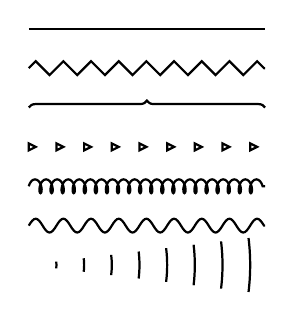
\begin{tikzpicture}[thick]
  \draw                                                (0,3)   -- (3,3);
  \draw[decorate,decoration=zigzag]                    (0,2.5) -- (3,2.5);
  \draw[decorate,decoration=brace]                     (0,2)   -- (3,2);
  \draw[decorate,decoration=triangles]                 (0,1.5) -- (3,1.5);
  \draw[decorate,decoration={coil,segment length=4pt}] (0,1)   -- (3,1);
  \draw[decorate,decoration={coil,aspect=0}]           (0,.5)  -- (3,.5);
  \draw[decorate,decoration={expanding waves,angle=7}] (0,0)   -- (3,0);
\end{tikzpicture}
\end{codeexample}

\begin{codeexample}[]
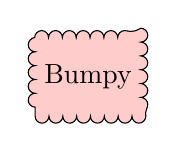
\begin{tikzpicture}
  \node [fill=red!20,draw,decorate,decoration={bumps,mirror},
         minimum height=1cm]
  {Bumpy};
\end{tikzpicture}
\end{codeexample}

\begin{codeexample}[]
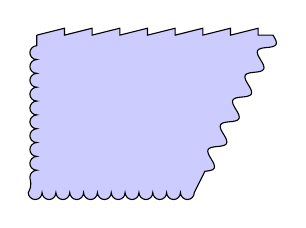
\begin{tikzpicture}
  \filldraw[fill=blue!20]                    (0,3)
  decorate [decoration=saw]             { -- (3,3) }
  decorate [decoration={coil,aspect=0}] { -- (2,1) }
  decorate [decoration=bumps]           { -| (0,3) };
\end{tikzpicture}
\end{codeexample}

\begin{codeexample}[]
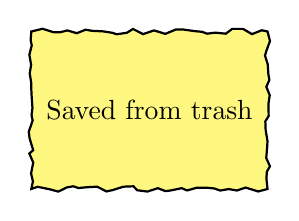
\begin{tikzpicture}
  \node [fill=yellow!50,draw,thick, minimum height=2cm, minimum width=3cm,
         decorate, decoration={random steps,segment length=3pt,amplitude=1pt}]
    {Saved from trash};
\end{tikzpicture}
\end{codeexample}

The general idea of decorations is the following: First, you construct a path
using the usual path construction commands. The resulting path is, in essence,
a series of straight and curved lines. Instead of directly using this path for
filling or drawing, you can then specify that it should form the basis for a
decoration. In this case, depending on which decoration you use, a new path is
constructed ``along'' the path you specified. For instance, with the |zigzag|
decoration, the new path is a zigzagging line that goes along the old path.

Let us have a look at an example: In the first picture, we see a path that
consists of a line, an arc, and a line. In the second picture, this path has
been used as the basis of a decoration.
%
\begin{codeexample}[]
\tikz \fill
  [fill=blue!20,draw=blue,thick] (0,0) -- (2,1) arc (90:-90:.5) -- cycle;
\end{codeexample}
%
\begin{codeexample}[]
\tikz \fill [decorate,decoration={zigzag}]
  [fill=blue!20,draw=blue,thick] (0,0) -- (2,1) arc (90:-90:.5) -- cycle;
\end{codeexample}

It is also possible to decorate only a subpath (the exact syntax will be
explained later in this section).
%
\begin{codeexample}[]
\tikz \fill [decoration={zigzag}]
  [fill=blue!20,draw=blue,thick] (0,0) -- (2,1)
    decorate { arc (90:-90:.5) } -- cycle;
\end{codeexample}

The |zigzag| decoration will be called a \emph{path morphing} decoration
because it morphs a path into a different, but topologically equivalent path.
Not all decorations are path morphing; rather there are three kinds of
decorations.

\begin{enumerate}
    \item The just-mentioned \emph{path morphing} decorations morph the path in
        the sense that what used to be a straight line might afterwards be a
        squiggly line or might have bumps. However, a line is still and a line
        and path deforming decorations do not change the number of subpaths.

        Examples of such decorations are the |snake| or the |zigzag|
        decoration. Many such decorations are defined in the library
        |decorations.pathmorphing|.

    \item \emph{Path replacing} decorations completely replace the path by a
        different path that is only ``loosely based'' on the original path. For
        instance, the |crosses| decoration replaces a path by a path consisting
        of a sequence of crosses. Note how in the following example filling the
        path has no effect since the path consist only of (numerous)
        unconnected straight line subpaths:
        %
\begin{codeexample}[]
\tikz \fill [decorate,decoration={crosses}]
  [fill=blue!20,draw=blue,thick] (0,0) -- (2,1) arc (90:-90:.5) -- cycle;
\end{codeexample}

        Examples of path replacing decorations are |crosses| or |ticks| or
        |shape backgrounds|. Such decorations are defined in the library
        |decorations.pathreplacing|, but also in |decorations.shapes|.
    \item \emph{Path removing} decorations completely remove the
        to-be-decorated path. Thus, they have no effect on the main path that
        is being constructed. Instead, they typically have numerous \emph{side
        effects}. For instance, they might ``write some text'' along the
        (removed) path or they might place nodes along this path. Note that for
        such decorations the path usage command for the main path have no
        influence on how the decoration looks like.
        %
\begin{codeexample}[]
\tikz \fill [decorate,decoration={text along path,
               text=This is a text along a path. Note how the path is lost.}]
  [fill=blue!20,draw=blue,thick] (0,0) -- (2,1) arc (90:-90:.5) -- cycle;
\end{codeexample}
        %
\end{enumerate}

Decorations are defined in different decoration libraries, see
Section~\ref{section-library-decorations} for details. It is also possible to
define your own decorations, see Section~\ref{section-base-decorations}, but
you need to use the \pgfname\ basic layer and a bit of theory is involved.

Decorations can be used to decorate already decorated paths. In the following
three graphics, we start with a simple path, then decorate it once, and then
decorate the decorated path once more.
%
\begin{codeexample}[]
\tikz \fill [fill=blue!20,draw=blue,thick]
  (0,0) rectangle (3,2);
\end{codeexample}
%
\begin{codeexample}[]
\tikz \fill [fill=blue!20,draw=blue,thick]
  decorate[decoration={zigzag,segment length=10mm,amplitude=2.5mm}]
    { (0,0) rectangle (3,2) };
\end{codeexample}
%
\begin{codeexample}[]
\tikz \fill [fill=blue!20,draw=blue,thick]
  decorate[decoration={crosses,segment length=2mm}] {
    decorate[decoration={zigzag,segment length=10mm,amplitude=2.5mm}] {
      (0,0) rectangle (3,2)
    }
  };
\end{codeexample}

One final word of warning: Decorations can be pretty slow to typeset and they
can be inaccurate. The reason is that \pgfname\ has to a \emph{lot} of rather
difficult computations in the background and \TeX\ is not very good at doing
math. Decorations are fastest when applied to straight line segments, but even
then they are much slower than other alternatives. For instance, the |ticks|
decoration can be simulated by clever use of a dashing pattern and the dashing
pattern will literally be thousands of times faster to typeset. However, for
most decorations there are no real alternatives.

\begin{tikzlibrary}{decorations}
    In order to use decorations, you first have to load a decoration library.
    This |decoration| library defines the basic options described in the
    following, but it does not define any new decorations. This is done by
    libraries like |decorations.text|. Since these more specialized libraries
    include the |decoration| library automatically, you usually do not have to
    bother about it.
\end{tikzlibrary}


\subsection{Decorating a Subpath Using the Decorate Path Command}

The most general way to decorate a (sub)path is the following path command.

\begin{pathoperation}{decorate}{\opt{\oarg{options}}\marg{subpath}}
    This path operation causes the \meta{subpath} to be decorated using the
    current decoration. Depending on the decoration, this may or may not extend
    the current path.
    %
\begin{codeexample}[]
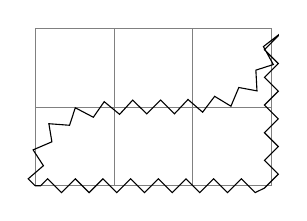
\begin{tikzpicture}
  \draw [help lines] grid (3,2);
  \draw decorate [decoration={name=zigzag}]
         { (0,0) .. controls (0,2) and (3,0) .. (3,2) |- (0,0) };
\end{tikzpicture}
\end{codeexample}
    %
    The path can include straight lines, curves, rectangles, arcs, circles,
    ellipses, and even already decorated paths (that is, you can nest
    applications of the |decorate| path command, see below).

    Due to the limits on the precision in  \TeX, some inaccuracies in
    positioning when crossing input segment boundaries may occasionally be
    found.

    You can use nodes normally inside the \meta{subpath}.
    %
\begin{codeexample}[]
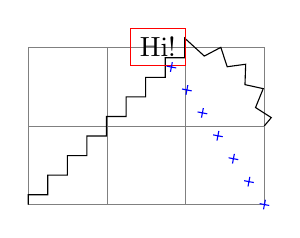
\begin{tikzpicture}
  \draw [help lines] grid (3,2);
  \draw decorate [decoration={name=zigzag}]
    { (0,0) -- (2,2) node (hi) [left,draw=red] {Hi!} arc(90:0:1)};

  \draw [blue] decorate [decoration={crosses}] {(3,0) -- (hi)};
\end{tikzpicture}
\end{codeexample}

    The following key is used to select the decoration and also to select
    further ``rendering options'' for the decoration.

    \begin{key}{/pgf/decoration=\meta{decoration options}}
            \keyalias{tikz}
        This option is used to specify which decoration is used and how it will
        look like. Note that this key will \emph{not} cause any decorations to
        be applied, immediately. It takes the |decorate| path command or the
        |decorate| option to actually decorate a path. The |decoration| option
        is only used to specify which decoration should be used, in principle.
        You can also use this option at the beginning of a picture or a scope
        to specify the decoration to be used with each invocation of the
        |decorate| path command. Naturally, any local options of the |decorate|
        path command override these ``global'' options.
        %
\begin{codeexample}[]
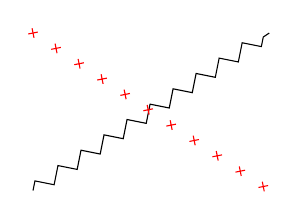
\begin{tikzpicture}[decoration=zigzag]
  \draw       decorate                      {(0,0) -- (3,2)};
  \draw [red] decorate [decoration=crosses] {(0,2) -- (3,0)};
\end{tikzpicture}
\end{codeexample}

        The \meta{decoration options} are special options (which have the path
        prefix |/pgf/decoration/|) that determine the properties of the
        decoration. Which options are appropriate for a decoration strongly
        depend on the decoration, you will have to look up the appropriate
        options in the documentation of the decoration, see
        Section~\ref{section-library-decorations}.

        There is one option (available only in \tikzname) that is special:
        %
        \begin{key}{/pgf/decoration/name=\meta{name} (initially none)}
            Use this key to set which decoration is to be used. The \meta{name}
            can both be a decoration or a meta-decoration (you need to worry
            about the difference only if you wish to define your own
            decorations).

            If you set \meta{name} to |none|, no decorations are added.
            %
\begin{codeexample}[]
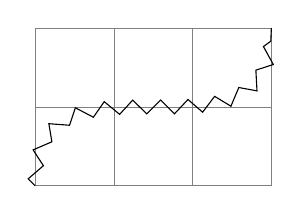
\begin{tikzpicture}
  \draw [help lines] grid (3,2);
  \draw decorate [decoration={name=zigzag}]
         { (0,0) .. controls (0,2) and (3,0) .. (3,2) };
\end{tikzpicture}
\end{codeexample}
            %
            Since this option is used so often, you can also leave out the
            |name=| part. Thus, the above example can be rewritten more
            succinctly:
            %
\begin{codeexample}[]
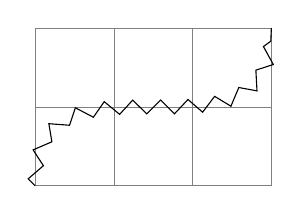
\begin{tikzpicture}
  \draw [help lines] grid (3,2);
  \draw decorate [decoration=zigzag]
         { (0,0) .. controls (0,2) and (3,0) .. (3,2) };
\end{tikzpicture}
\end{codeexample}
            %
            In general, when \meta{decoration options} are parsed, for each
            unknown key it is checked whether that key happens to be a
            (meta-)decoration and, if so, the |name| option is executed for
            this key.
        \end{key}

        Further options allow you to adjust the position of decorations
        relative to the to-be-decorated path. See
        Section~\ref{section-decorations-adjust} below for details.
    \end{key}

    Recall that some decorations actually completely remove the to-be-decorated
    path. In such cases, the construction of the main path is resumed after the
    |decorate| path command ends.
    %
\begin{codeexample}[]
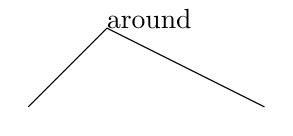
\begin{tikzpicture}[decoration={text along path,text=
      around and around and around and around we go}]

  \draw (0,0) -- (1,1) decorate { -- (2,1) } -- (3,0);
\end{tikzpicture}
\end{codeexample}

    It is permissible to nest |decorate| commands. In this case, the path
    resulting from the first decoration process is used as the to-be-decorated
    path for the second decoration process. This is especially useful for
    drawing fractals. The |Koch snowflake| decoration replaces a straight line
    like \tikz\draw (0,0) -- (1,0); by
    \tikz[decoration=Koch snowflake] \draw decorate{(0,0) -- (1,0)};.
    Repeatedly applying this transformation to a triangle yields a fractal that
    looks a bit like a snowflake, hence the name.
    %
\begin{codeexample}[]
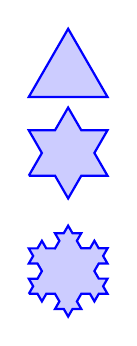
\begin{tikzpicture}[decoration=Koch snowflake,draw=blue,fill=blue!20,thick]
  \filldraw (0,0) -- ++(60:1) -- ++(-60:1) -- cycle ;
  \filldraw decorate{ (0,-1) -- ++(60:1) -- ++(-60:1) -- cycle };
  \filldraw decorate{ decorate{ (0,-2.5) -- ++(60:1) -- ++(-60:1) -- cycle }};
\end{tikzpicture}
\end{codeexample}
    %
\end{pathoperation}


\subsection{Decorating a Complete Path}

You may sometimes wish to decorate a path over whose construction you have no
control. For instance, the path of the background of a node is created without
having a chance to issue a |decorate| path command. In such cases you can use
the following option, which allows you to decorate a path ``after the fact''.

\begin{key}{/tikz/decorate=\opt{\meta{boolean}} (default true)}
    When this key is set, the whole path is decorated after it has been
    finished. The decoration used for decorating the path is set via the
    |decoration| way, in exactly the same way as for the |decorate| path
    command. Indeed, the following two commands have the same effect:
    %
    \begin{enumerate}
        \item |\path decorate[|\meta{options}|] {|\meta{path}|};|
        \item |\path [decorate,|\meta{options}|] |\meta{path}|;|
    \end{enumerate}
    %
    The main use or the |decorate| option is the you can also use it with the
    nodes. It then causes the background path of the node to be decorated. Note
    that you can decorate a background path only once in this manner. That is,
    in contrast to the |decorate| path command you cannot apply this option
    twice (this would just set it to |true|, once more).
    %
\begin{codeexample}[preamble={\usetikzlibrary{shapes.geometric}}]
\begin{tikzpicture}[decoration=zigzag]
  \draw [help lines] (0,0) grid (3,5);

  \draw [fill=blue!20,decorate] (1.5,4) circle (1cm);

  \node at (1.5,2.5) [fill=red!20,decorate,ellipse] {Ellipse};

  \node at (1.5,1) [inner sep=6mm,fill=red!20,decorate,ellipse,decoration=
    {text along path,text={This is getting silly}}] {Ellipse};
\end{tikzpicture}
\end{codeexample}

    In the last example, the |text along path| decoration removes the path. In
    such cases it is useful to use a pre- or postaction to cause the decoration
    to be applied only before or after the main path has been used.
    Incidentally, this is another application of the |decorate| option that you
    cannot achieve with the decorate path command.
    %
\begin{codeexample}[preamble={\usetikzlibrary{shapes.geometric}}]
\begin{tikzpicture}[decoration=zigzag]
  \node at (1.5,1) [inner sep=6mm,fill=red!20,ellipse,
    postaction={decorate,decoration=
    {text along path,text={This is getting silly}}}] {Ellipse};
\end{tikzpicture}
\end{codeexample}
    %
    Here is more useful example, where a postaction is used to add the path
    after the main path has been drawn.
    %
% \catcode`\|12 % !?
\begin{codeexample}[]
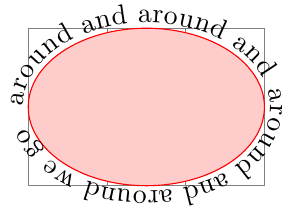
\begin{tikzpicture}
\draw [help lines] grid (3,2);
\fill [draw=red,fill=red!20,
         postaction={decorate,decoration={raise=2pt,text along path,
           text=around and around and around and around we go}}]
  (0,1) arc (180:-180:1.5cm and 1cm);
\end{tikzpicture}
\end{codeexample}
    %
\end{key}


\subsection{Adjusting Decorations}
\label{section-decorations-adjust}

\subsubsection{Positioning Decorations Relative to the To-Be-Decorate Path}

The following option, which are only available with \tikzname, allow you to
modify the positioning of decorations relative to the to-be-decorated path.

\begin{key}{/pgf/decoration/raise=\meta{dimension} (initially 0pt)}
    The segments of the decoration are raised by \meta{dimension} relative to
    the to-be-decorated path. More precisely, the segments of the path are
    offset by this much ``to the left'' of the path as we travel along the
    path. This raising is done after and in addition to any transformations set
    using the |transform| option (see below).

    A negative \meta{dimension} will offset the decoration ``to the right'' of
    the to-be-decorated path.
    %
\begin{codeexample}[]
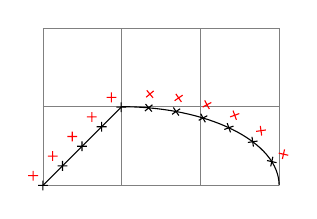
\begin{tikzpicture}
  \draw [help lines] (0,0) grid (3,2);

  \draw (0,0) -- (1,1) arc (90:0:2 and 1);
  \draw      decorate [decoration=crosses]
        { (0,0) -- (1,1) arc (90:0:2 and 1) };
  \draw[red] decorate [decoration={crosses,raise=5pt}]
        { (0,0) -- (1,1) arc (90:0:2 and 1) };
\end{tikzpicture}
\end{codeexample}
    %
\end{key}

\begin{key}{/pgf/decoration/mirror=\opt{\meta{boolean}}}
    Causes the segments of the decoration to be mirrored along the
    to-be-decorated path. This is done after and in addition to any
    transformations set using the |transform| and/or |raise| options.
    %
\begin{codeexample}[]
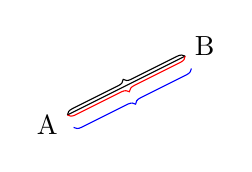
\begin{tikzpicture}
  \node (a)          {A};
  \node (b) at (2,1) {B};
  \draw                                                    (a) -- (b);
  \draw[decorate,decoration=brace]                         (a) -- (b);
  \draw[decorate,decoration={brace,mirror},red]            (a) -- (b);
  \draw[decorate,decoration={brace,mirror,raise=5pt},blue] (a) -- (b);
\end{tikzpicture}
\end{codeexample}
    %
\end{key}

\begin{key}{/pgf/decoration/transform=\meta{transformations}}
    This key allows you to specify general \meta{transformations} to be applied
    to the segments of a decoration. These transformations are applied before
    and independently of |raise| and |mirror| transformations. The
    \meta{transformations} should be normal \tikzname\ transformations like
    |shift| or |rotate|.

    In the following example the |shift only| transformation is used to make
    sure that the crosses are \emph{not} sloped along the path.
    %
\begin{codeexample}[]
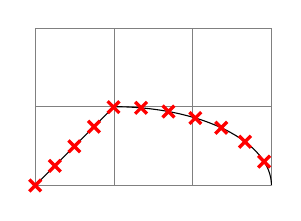
\begin{tikzpicture}
  \draw [help lines] (0,0) grid (3,2);

  \draw (0,0) -- (1,1) arc (90:0:2 and 1);
  \draw[red,very thick] decorate [decoration={
               crosses,transform={shift only},shape size=1.5mm}]
        { (0,0) -- (1,1) arc (90:0:2 and 1) };
\end{tikzpicture}
\end{codeexample}
    %
\end{key}


\subsubsection{Starting and Ending Decorations Early or Late}

You sometimes may wish to ``end'' a decoration a bit early on the path. For
instance, you might wish a |snake| decoration to stop 5mm before the end of the
path and to continue in a straight line. There are different ways of achieving
this effect, but the easiest may be the |pre| and |post| options, which only
have an effect in \tikzname. Note, however, that they can only be used with
decorations, not with meta-decorations.

\begin{key}{/pgf/decoration/pre=\meta{decoration} (initially lineto)}
    This key sets a decoration that should be used before the main decoration
    starts. The \meta{decoration} will be used for a length of |pre length|,
    which |0pt| by default. Thus, for the |pre| option to have any effect, you
    also need to set the |pre length| option.
    %
    % TODO: Nesting tikzpictures is NOT supported
\begin{codeexample}[]
\tikz [decoration={zigzag,pre=lineto,pre length=1cm}]
  \draw [decorate] (0,0) -- (2,1) arc (90:0:1);
\end{codeexample}
    %
\begin{codeexample}[]
\tikz [decoration={zigzag,pre=moveto,pre length=1cm}]
  \draw [decorate] (0,0) -- (2,1) arc (90:0:1);
\end{codeexample}
    %
\begin{codeexample}[]
\tikz [decoration={zigzag,pre=crosses,pre length=1cm}]
  \draw [decorate] (0,0) -- (2,1) arc (90:0:1);
\end{codeexample}

    Note that the default |pre| option is |lineto|, not |curveto|. This means
    that the default |pre| decoration will not follow curves (for efficiency
    reasons). Change the |pre| key to |curveto| if you have a curved path.
    %
\begin{codeexample}[]
\tikz [decoration={zigzag,pre length=3cm}]
  \draw [decorate] (0,0) -- (2,1) arc (90:0:1);
\end{codeexample}
    %
\begin{codeexample}[]
\tikz [decoration={zigzag,pre=curveto,pre length=3cm}]
  \draw [decorate] (0,0) -- (2,1) arc (90:0:1);
\end{codeexample}
    %
\end{key}

\begin{key}{/pgf/decoration/pre length=\meta{dimension} (initially 0pt)}
    This key sets the distance along which the pre-decoration should be used.
    If you do not need/wish a pre-decoration, set this key to |0pt| (exactly
    this string, not just to something that evaluates to the same things such
    as |0cm|).
\end{key}

\begin{key}{/pgf/decorations/post=\meta{decoration} (initially lineto)}
    Works like |pre|, only for the end of the decoration.
\end{key}

\begin{key}{/pgf/decorations/post length=\meta{dimension} (initially 0pt)}
    Works like |pre length|, only for the end of the decoration.
\end{key}

Here is a typical example that shows how these keys can be used:
%
\begin{codeexample}[]
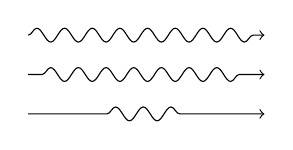
\begin{tikzpicture}
  [decoration=snake,
   line around/.style={decoration={pre length=#1,post length=#1}}]

  \draw[->,decorate]                  (0,0)    -- ++(3,0);
  \draw[->,decorate,line around=5pt]  (0,-5mm) -- ++(3,0);
  \draw[->,decorate,line around=1cm]  (0,-1cm) -- ++(3,0);
\end{tikzpicture}
\end{codeexample}
